\documentclass[10pt]{article}
\usepackage[margin=0.8in]{geometry}
\usepackage{amsmath,amssymb,graphicx,booktabs,tabularx,hyperref}
\hypersetup{colorlinks=true,urlcolor=blue}
\setlength{\parindent}{0pt}
\setlength{\parskip}{6pt}
\title{Four APS follow-up leads: implementation and correctness}
\author{}
\date{28 October 2026}
\begin{document}
\maketitle
\textbf{Scope.} Native bounded development checks, not a performance result.
\par Baseline: \path{6187036c049b6de2b1521b014f575952e4f1705c}.
The earlier APS implementation is
\href{https://github.com/isogeny-labs/crypto/pull/2614}{PR 2614}.

\textbf{1. Verified early termination.}
The new visitor receives roots only after evaluation against the original
equations. Coordinates are decoded and deduplicated before checking actual
signed point sums, known labels, $B\ne0$, and $dG=Q$.
Uninformative roots do not stop the search. Hybrid guesses and covering
partitions share a cooperative deadline and stop on the verified witness.
A stopped search explicitly reports partial enumeration; it is distinct from
complete exhaustion and timeout. Exhaustive mode and the legacy full-field
solver remain available as controls.

\textbf{2. Membership-aware root extraction.}
Coordinate variables carry exact finite domains generated together with
their vanishing equations. Substitution preserves the domain's original
variable identity. Auxiliary, elementary-symmetric and line parameters
remain unrestricted. Their univariates use the existing counted
$\gcd(f,X^p-X)$ and Cantor--Zassenhaus implementation with cancellation.
If there is no univariate, full-field fallback remains possible and explicit.
The field cap stays $p\le65521$. Root diagnostics are stage observations;
they omit other costs and cannot establish a complete-cost gain.

\textbf{3. Two-parameter line selection.}
For $E:y^2=x^3+ax+b$ and $y=tx+c$, substitution gives
\[
 H_{t,c}(X)=X^3-t^2X^2+(a-2tc)X+b-c^2.
\]
The three remainder equations for $H_{t,c}\mid F_V$ select distinct base
coordinates. This uses two parameters instead of three elementary symmetric
coordinates plus the symmetric $S_3$ equation. It is the standard chord
construction, not a novelty claim. Fewer variables can produce harder
remainder equations; no speed or degree improvement follows automatically.

\textbf{4. Certified orbit-component removal.}
On $j=0$, horizontal lines select full order-three automorphism orbits.
When labels are propagated by an eigenvalue $\lambda$ satisfying
$1+\lambda+\lambda^2=0$, both label sums vanish. After checking orbit closure,
point labels, sign changes, and eigenvalue action on both $G$ and $Q$, the
builder adds $tz-1=0$ to exclude those components. Independently labeled
points on the same geometric orbit can be informative and are refused by
this pruning builder. The ordinary $B=0$ guard remains in recovery.
The inverse variable can increase elimination cost; pruning is not an
automatic speed improvement.

\newpage
\begin{center}
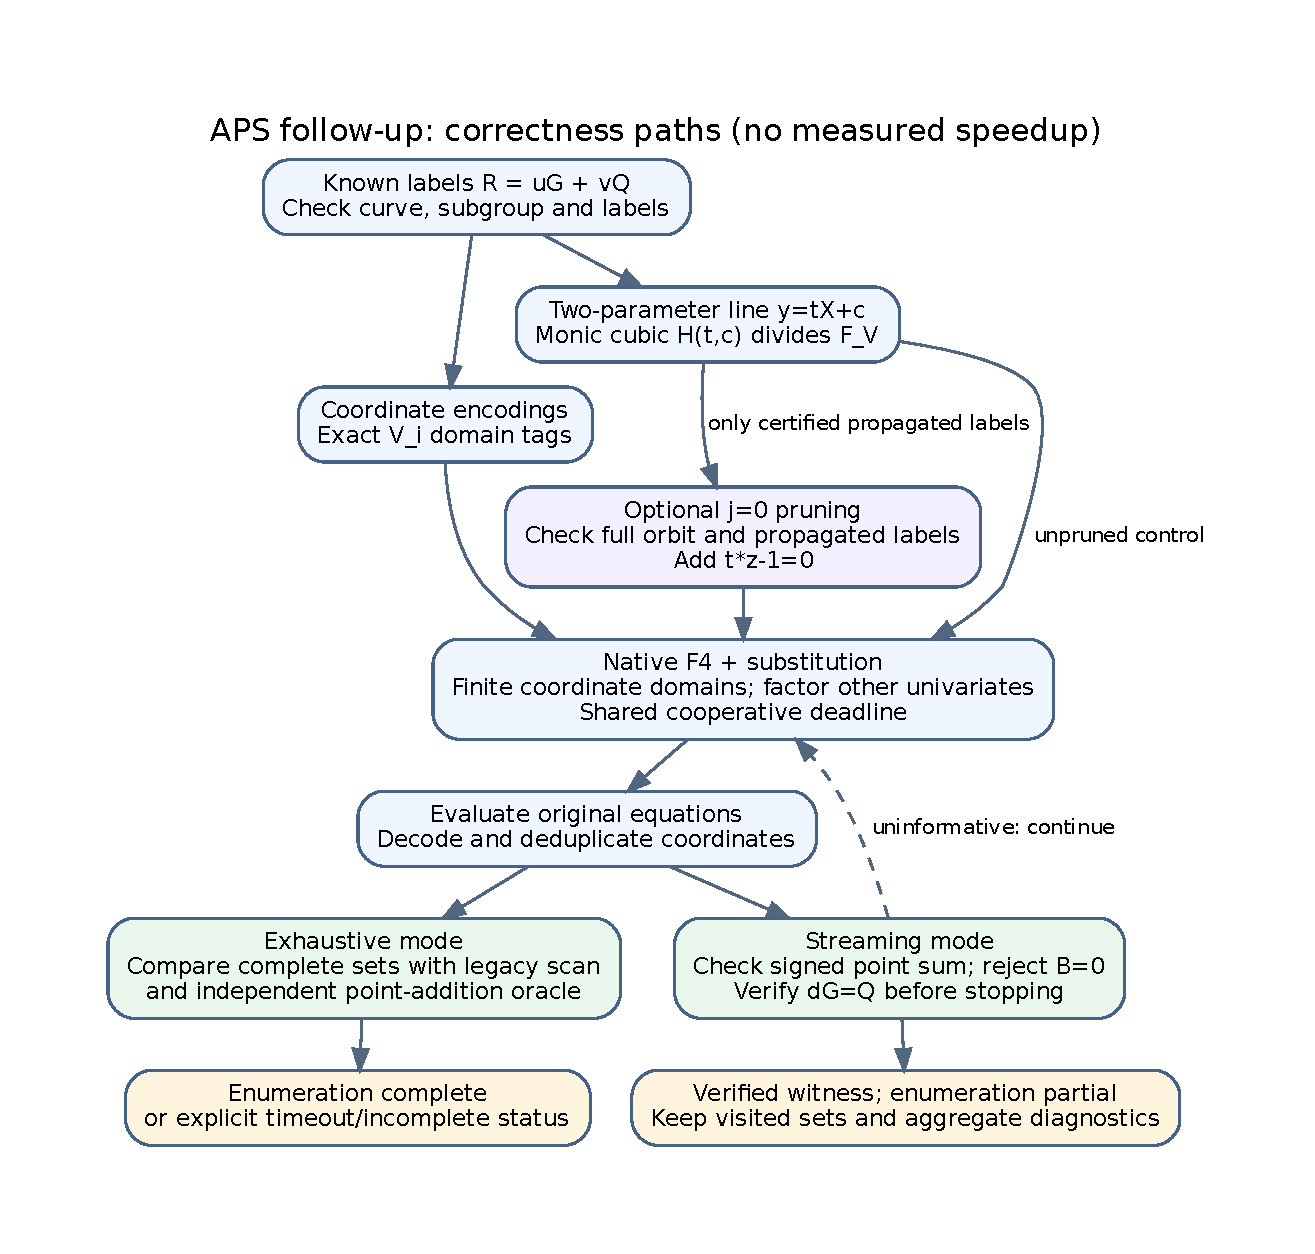
\includegraphics[width=0.94\linewidth,height=0.54\textheight,keepaspectratio]{pipeline.pdf}
\end{center}
\textbf{Verification and limits.}
The final command receipts and requirement status are in the study README
and \texttt{validation/}. Seven core-only Lean lemmas cover coefficient
expansion, root soundness, sign invariance, orbit-label cancellation and
conditional saturation. Their axioms are standard. The full squarefree
divisor/chord-law completeness theorem, subgroup sign argument, and Rust
correspondence remain a partial formalization; see \texttt{PROOF\_MAP.md}.

The full release suite passed 5,002 tests, with zero failures and 122
existing ignored tests. Focused checks passed 20 APS, 7 CLI, 63 F4-related
and 15 GLV tests. They compare exact relation sets, verify known public
answers and test refusal/timeout cases. They share the native curve
arithmetic; independent EC replay remains open.
The shipped native identity certificate is
\path{IDC1h0abc57c4d1e81eb0}; the example checks its statement fingerprint
and evaluates a second seeded set of points. See \path{line-identity.json}.

\textbf{Performance remains open.}
No end-to-end cost, external solver comparison, speedup or scaling is
measured. Complete accounting/replay/export and a frozen controlled protocol
are still owed in the
\href{https://github.com/isogeny-labs/crypto/tree/main/backlog/XP-20261026-aps-complete-cost-panel}{existing complete-cost panel}.
Automatic approval review rejected the mandatory resume checkpoint upload
because it would package source and local changes for S3; no performance
experiment was launched or checkpoint gate bypassed. Local correctness
checks and publication of the requested PR proceed separately.

\textbf{Sources.}
\href{https://eprint.iacr.org/2017/609}{Amadori--Pintore--Sala (2018)},
revised manuscript, sections 3.1--3.4;
\href{https://www.jmilne.org/math/Books/EC2.pdf}{Milne, Elliptic Curves,
second edition}, I section 3;
\texttt{research/factor\_base\_designs\_20261015/README.md}, design 11
(including its cost-unfavourable measured cases);
\texttt{src/cryptanalysis/glv\_invariant\_base.rs}, existing root extraction.
The earlier source map records the Kudo follow-up full-text access gap;
no reproduction or novelty claim depends on that inaccessible body.

The IC leaderboard, performance charts and canonical curve graphs receive
no new values: this study establishes no qualifying measured gain or new
curve route. The editable diagram above records the implemented paths.
\end{document}
